% Définition du nom du chapitre
\chapter[Fine-scale automatic mapping of living \textit{Posidonia oceanica} seagrass beds with underwater photogrammetry]{Chapitre 3: Fine-scale automatic mapping of living \textit{Posidonia oceanica} seagrass beds with underwater photogrammetry} \label{chapitre3-herbiers}

\pagestyle{main}

%%%%%%%%%%%%%%%%%%%%%%%%%%%%%
%%% Figure cover chapitre %%%
%%%%%%%%%%%%%%%%%%%%%%%%%%%%%
\begin{tikzpicture}
  \def\ig{%
   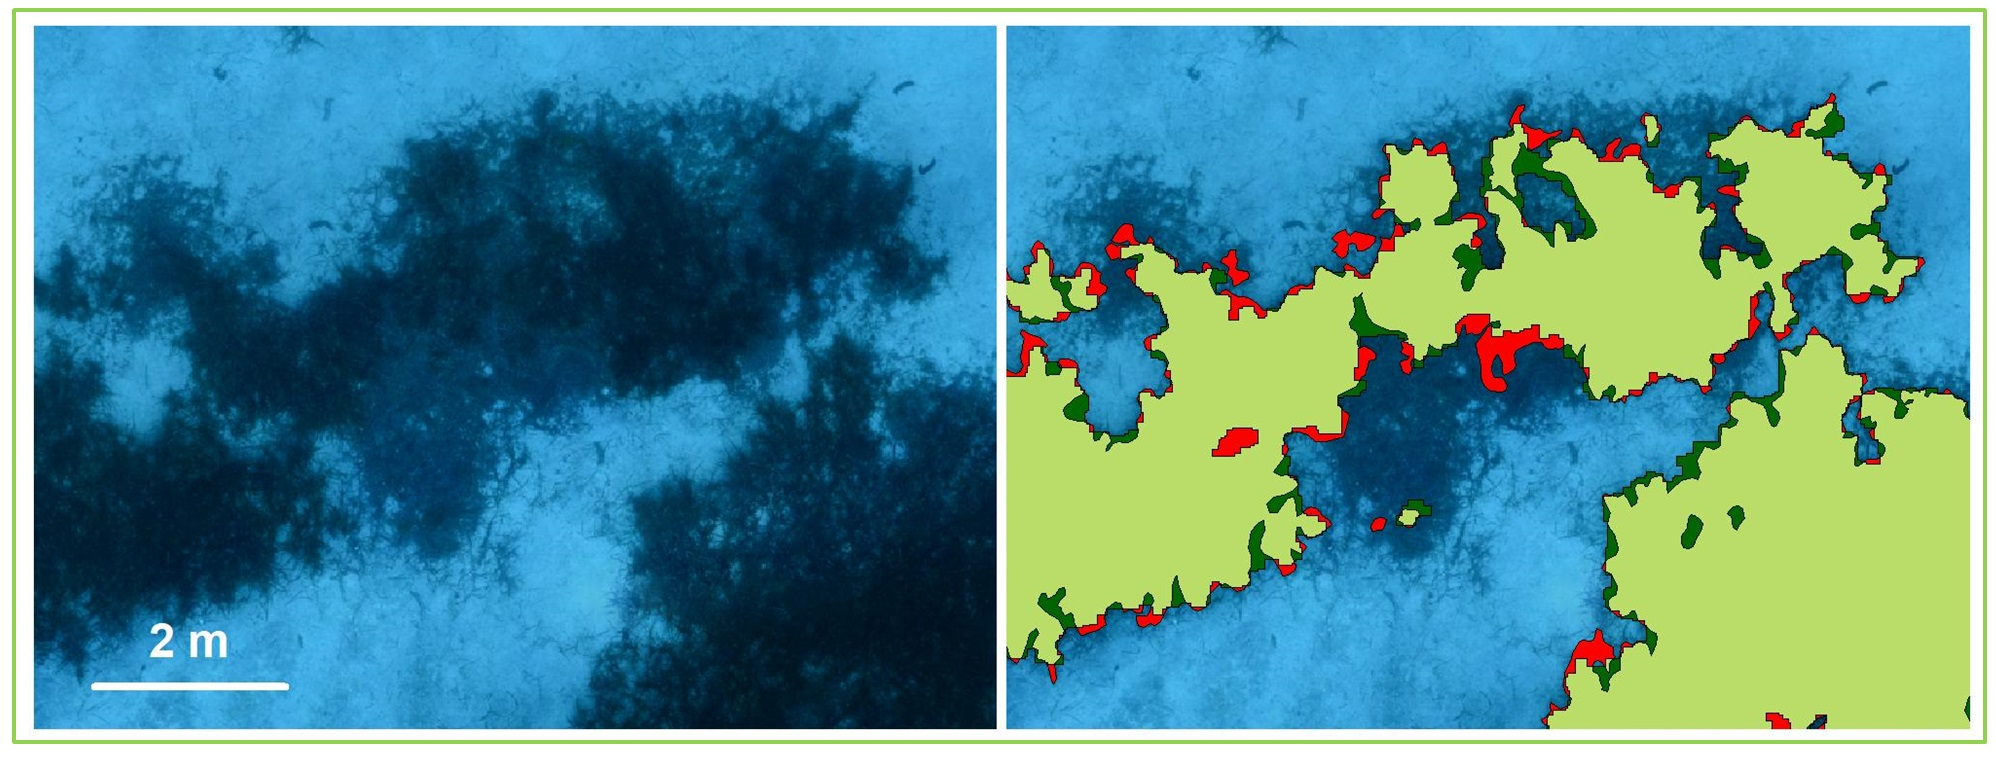
\includegraphics[width=\linewidth,keepaspectratio]{./5_chapitre3/cover.jpg}}
 \node [inner sep=0pt](mypicture) at (0,0) {\phantom{\ig}};
 \clip[rounded corners=5mm] ($(mypicture.south west)+(\bord,\bord)$) rectangle ($(mypicture.north east)-(\bord,\bord)$);
 \node[inner sep=0pt](mypicture) at (0,0) {\ig};
\end{tikzpicture}

% Bullet points du début de chapitre
\begin{center}
\begin{colbox}{resume}
  \vspace{-2pt}
{\color{textresume}\small
\begin{itemize}[leftmargin=0in]\itemsep3pt
\item \textbf{OBJECTIFS}~:
    \begin{itemize}
      \item Mise au point d'une \textbf{méthode de cartographie} automatique des herbiers de Posidonie par \textbf{photogrammétrie}~;
      \item \textbf{Application} de la méthode pour des suivis d'herbiers en limite inférieure~;
    \end{itemize}
\item \textbf{RESULTATS}~:
    \begin{itemize}
      \item La \textbf{précision}, le \textbf{taux de rappel} et le \textbf{F1-score} moyens sur 21 sites sont respectivement de \textbf{0.79, 0.91} et \textbf{0.84}~;
      \item La \textbf{profondeur}, le \textbf{type de substrat}, la \textbf{surface} de la zone d'étude ainsi que la \textbf{densité} de l'herbier n'ont pas d'influence significative sur la précision de la méthode~;
      \item Le niveau de \textbf{fragmentation} de l'herbier affecte significativement la qualité de la classification.
      \item L'application de la méthode pour le \textbf{suivi} de trois herbiers en limite inférieure montre \textbf{l'opérabilité} de la méthode et la \textbf{progression} des sites sur une période de 3 ans.
    \end{itemize}
\end{itemize}
}
\vspace{-2pt}
\end{colbox}
\end{center}

\clearpage

\noindent\textbf{Fine-scale automatic mapping of living \textit{Posidonia oceanica} seagrass beds with underwater photogrammetry}

% Auteurs
%\noindent Guilhem Marre, Florian Holon, Sandra Luque, Pierre Boissery et Julie Deter

% NB sans indentation
\noindent\href{https://doi.org/10.3354/meps13338}{\textit{Marre G, Deter J, Holon F, Boissery P and Luque S (2020) Fine-scale automatic mapping of living \textit{Posidonia oceanica} seagrass beds with underwater photogrammetry. Marine Ecology Progress Series XXX. doi: https://doi.org/10.3354/meps13338}}

\medskip

\noindent\textbf{Abstract}
The Mediterranean seagrass \textit{Posidonia oceanica}, which provides highly valuable ecosystem services, is subject to increasing anthropogenic pressures, causing habitat loss or fragmentation. Whilst airborne images and acoustic data can be used for monitoring seagrass coverage at a macro-scale and over large periods of time, monitoring its health in the short-term requires precision mapping in order to assess current regression / progression of the meadow. However, currently used fine-scale underwater techniques are imprecise and time demanding in the field. We propose an automatic classification approach based on underwater photogrammetry for an operational, cost and time effective fine-scale monitoring method. The method uses a property of the sparse cloud generated during bundle adjustment, the reconstruction uncertainty, to map seagrass patches. The mean precision, recall, and F1 score of the method over 21 study sites with different morphologies were: 0.79, 0.91 and 0.84, respectively. However, the fragmentation level of the meadows had a significant negative effect on classification performances. The temporal monitoring of three sites using this method has proven its operability and showed a positive evolution index of the corresponding meadows over a period of three years. This method is generalizable for most encountered configurations and can be integrated in a large monitoring system, as it enables the production of numerous seagrass maps over a short period of time. Moreover, our methodology could be generalized and applied in the study of other submerged aquatic vegetation, by adjusting the method’s parameters.

\noindent\textbf{Keywords}
\textit{Posidonia oceanica}, underwater photogrammetry, benthic habitat mapping, monitoring, reconstruction uncertainty, submerged aquatic vegetation

% Introduction
\section{Introduction}\label{chapitre3_1}
At the global scale, ecosystems are threatened by numerous anthropogenic pressures \citep{hoekstra_confronting_2004, halpern_global_2008} and the consequent habitat loss and fragmentation are known to have a considerable impact on their biodiversity \citep{brooks_habitat_2002, haddad_habitat_2015}. Marine ecosystems, notably coastal ecosystems, are not exempt from the impacts of human activities, since they host high levels of marine biodiversity \citep{halpern_global_2008} competing with a human population density of about three times the average elsewhere \citep{small_global_2003}. Seagrass meadows, in particular, provide important and valuable ecosystem services and are responsible for more than half of the total value of the world’s natural capital and services \citep{costanza_value_1997, millenium_ecosystem_assessment_ecosystem_2005, ipbes_global_2019}. \textit{Posidonia oceanica}, a protected species of seagrass which is endemic to the Mediterranean Sea, is under threat from the coastal human population and steadily increasing rates of man-made coastline \citep{holon_impact_2015, holon_predictive_2018}, which are responsible for the fragmentation and destruction of this fragile habitat  \citep{montefalcone_human_2010, holon_impact_2015}. This species, which grows at depths ranging from surface-level to 44 m depending upon water clarity \citep{boudouresque_regression_2009}, is commonly used as a bioindicator because of its sensitivity to environmental disturbance, most notably evolutions of its lower limit (i.e. the deep edge of the meadow below which the most favourable conditions for the growing of \textit{P. oceanica} are no longer met) \citep{boudouresque_regression_2009, ruiz_mediterranean_2009}. Indeed, the lower limit of seagrasses is primarily determined by water clarity and delivers a robust indicator of the overall status for all species (Borum et al. 2004). Studies conducted at a macro scale have indicated a steady loss in shallow beds over the course of the 20th century \citep{marba_mediterranean_2014, holon_impact_2015}. Consequently, to complete these large-scale studies, precision mapping is required in order to monitor the lower limit at a fine scale and to quantify its spatial changes in the short term: progression (i.e. colonization) vs. regression (i.e. death and / or erosion). These dynamics must be correlated to local anthropogenic pressures, and results need to be extrapolated over larger areas to support decision makers on conservation decisions. For our findings to be integrated into a large-scale monitoring system, an effective method must be developed in order to anticipate microevolutions at its lower limit, and better engage with the relevant conservation policies.

In the past, various monitoring tools have been employed to survey the evolution of the lower limit of \textit{P. oceanica} \citep{noel_cahier_2012}. The Posidonia Monitoring Network (PMN) consists in placing permanent concrete blocks at the lower limit and regularly measuring the distance from the blocks to the seagrass’ lower limit, to assess linear progression / regression over time \citep{boudouresque_monitoring_2007, pergent_protocole_2007}. It is however a considerably intrusive procedure with a very low spatial resolution. An alternative method employs acoustic telemetry: a diver can create numerous points in order to accurately pinpoint the lower limit \citep{descamp_underwater_2005, descamp_fast_2011}. This method is relatively accurate, but the procedure is time consuming, and is subject to physiological constraints of the diver when working in the deepest meadows (i.e. 35 - 45 m). Spatial resolution (distance between points) is also subject to the diver’s discretion. Remote sensing could be considered a favourable option, but only for clear, shallow waters \citep{koedsin_integrated_2016, pu_mapping_2017, topouzelis_seagrass_2018, traganos_mapping_2018}. It is regrettably unsuitable for turbid waters and also darker and deeper conditions presented by the lower limit of \textit{P. oceanica}. We therefore propose a non-intrusive mapping protocol which incorporates underwater photogrammetry.

Underwater photogrammetry involves the virtual reconstruction of three-dimensional (3D) models and / or orthomosaics of the seafloor, by using numerous images. The images may be taken by a diver \citep{mizuno_simple_2017}; an Autonomous Underwater Vehicle (AUV) \citep{bryson_automated_2013, bonin-font_towards_2016}; a Remotely Operated Vehicle (ROV) \citep{drap_rov_2015}; or by a towed camera \citep{rende_advances_2015}. The technique has been deemed suitable for monitoring natural or anthropogenic disturbances and their effects on marine ecosystems \citep{burns_assessing_2016}, and has seen increasing application in the field of marine ecology. Previously, most studies which mapped seagrass beds using underwater photogrammetry produced an orthomosaic (orthorectified photo assemblage) of the seafloor, then built a classifier based either on luminance value \citep{mizuno_simple_2017} or on colorimetry and texture \citep{rende_advances_2015, bonin-font_towards_2016}. Some of these studies performed highly, achieving 95 \% accuracy \citep{bonin-font_towards_2016}, however, it should be noted that all classifiers were trained and optimized on a single study site, and accounted for neither morphological varieties, nor for variation in specific, underwater conditions. Moreover, the variability between meadows in terms of depth, substrate, and lighting conditions, makes it difficult to build an accurate and generalizable classifier based on colours or luminance. There is a need for an operational methodology that can automatically map seagrass meadows in different lighting conditions and site morphologies.

In this study, we tested an operational method for the centimetric mapping of \textit{P. oceanica} meadows in study sites ranging from 57 to 781 m², using underwater photogrammetry along the lower limits. The method uses datasets collected by a diver, and exploits reconstruction uncertainty; a property of the sparse cloud (3D point cloud composed of the tie points between all of the images) produced during bundle adjustment (alignment of the set of photos in the 3D space). Using 256 combinations of parameters, the workflow was designed, optimized, and tested in order to achieve the best classification accuracy over 21 study sites. Finally, the parametrized workflow was used to assess the evolution of the seagrass cover of three of the 21 study sites over the period 2016 - 2019.


% Material and methods
\section{Materials and methods}\label{chapitre3_2}

\subsection{Study sites}
The data was collected in June 2016, 2017 and 2019 along the French Mediterranean coast during the TEMPO monitoring network campaigns \citep{andromede-oceanologie_tempo_2020}. TEMPO is the largest French initiative for the monitoring of \textit{P. oceanica}’s ecological status and ecosystem along the French Mediterranean coast, from Spain to Italy, including the Corsican coast (see \autoref{figure3.1}). The network includes data collection for 47 sites located at 15 m (seagrass density and leaves length, grazing, fish abundance, filtering organisms…) and 53 lower limits (surface area evolution, density, shoot heaving, fish abundance,…). These data are collected and analysed in order to assess \textit{P. oceanica}’s ecological status and trend, investigate the correlations with environmental conditions and anthropogenic pressures to support decision makers build wise conservation policies.


%%%%%%%%%%%%%%%%%%%%%%%%%%%%%%%%%%%%%%%%%%%%%
%%% Figure 3.1: Study sites TEMPO network %%%
%%%%%%%%%%%%%%%%%%%%%%%%%%%%%%%%%%%%%%%%%%%%%
\begin{figure}[H]
	\begin{center}
	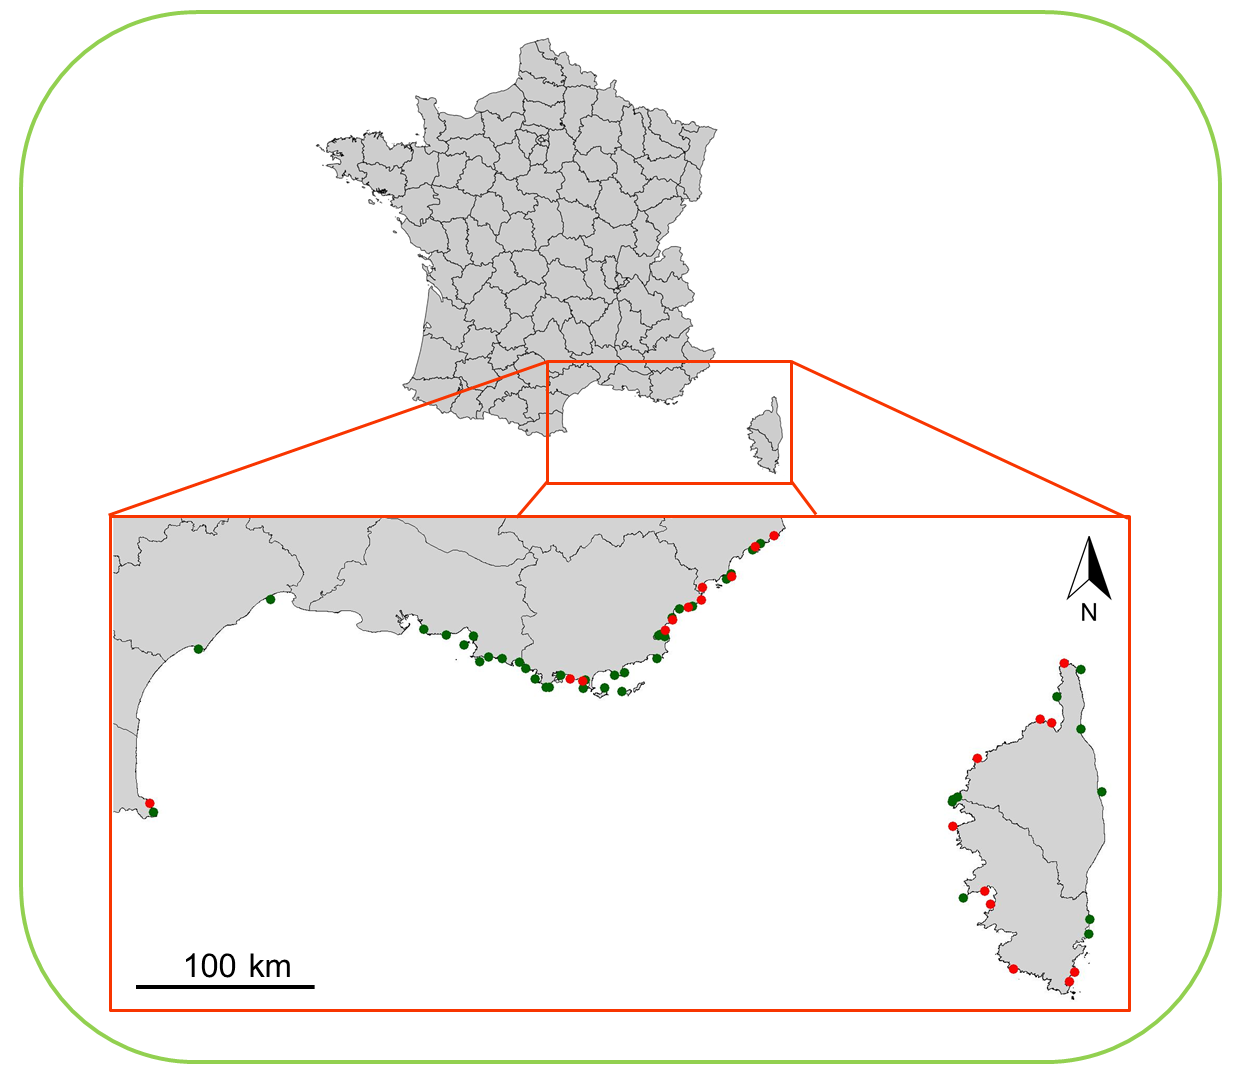
\includegraphics[width=\linewidth]{./5_chapitre3/Figure3.1}
		\caption[\textit{Posidonia oceanica}’s lower limit monitoring sites.]{\textit{Posidonia oceanica}’s lower limit monitoring sites (TEMPO monitoring network; South of France and Corsica). Red dots = localization of the 21 study sites; green dots = other sites of the network).}
	\label{figure3.1}
\end{center}
\end{figure}


We used the data from the lower limits of 21 \textit{Posidonia oceanica} beds, located between 13 and 37 m deep (see \autoref{figure3.1}). The large depth range allowed the assessment of various environmental conditions, including the more exposed, shallow sites, and darker, more sheltered, deep sites. Study areas ranged from 57 to 781 m² in size, and differed in the substrate type (mud / sand), fragmentation level (ratio perimeter / area) and shoot density (see \autoref{table3.1}).

%%%%%%%%%%%%%%%%%%%%%%%%%%%%%%%%%%%
%%% Table 3.1: Site properties  %%%
%%%%%%%%%%%%%%%%%%%%%%%%%%%%%%%%%%%
\begin{table}[H]
  \centering
  \normalsize
 % \raggedright
  \caption[Properties of the 21 study sites]{Properties of the 21 study sites. Fragmentation = perimeter / surface area of all patches. The shoot density was measured in-situ by hand within three 0.2 x 0.2 m quadrats and averaged}
  \label{table3.1}
    \begin{tabular}{*{6}{c}}
        \toprule
        \textbf{Site} & \makecell{\textbf{Depth} \\ \textbf{(m)}} & \textbf{Substrate} & \makecell{\textbf{Surface} \\ \textbf{(m²)}} & \textbf{Fragmentation} & \makecell{\textbf{Density} \\ \textbf{(shoots.m-²)}} \\ \midrule
        Agay Ouest & 24 & Sand & 177 & 2.24 & 245 \\
        Agriates & 37 & Sand & 499 & 2.43 & 233 \\
        Cap Gros Nord & 21 & Sand & 194 & 2.52 & 113 \\
        Cap Roux & 28 & Sand & 260 & 4.97 & 147 \\
        Cappo Rosso & 34 & Sand & 646 & 2.39 & 177 \\
        Carqueiranne & 29 & Mud & 212 & 12.30 & 154 \\
        Giraglia & 35 & Sand & 533 & 3.37 & 206 \\
        Golfe Santa Manza & 31 & Mud & 471 & 4.80 & 84 \\
        Isolella & 29 & Sand & 167 & 3.23 & 229 \\
        Murtoli & 31 & Sand & 426 & 2.06 & 261 \\
        Paulilles & 14 & Mud & 57 & 6.64 & 215 \\
        Plage Suveret & 13 & Mud & 96 & 4.15 & 170 \\
        Plage Trottel & 25 & Sand & 537 & 3.16 & 93 \\
        Pointe de la Calle & 24 & Mud & 113 & 8.78 & 113 \\
        Pointe Rube & 15 & Mud & 201 & 3.48 & 149 \\
        Pointe Veille Est & 25 & Sand & 201 & 2.45 & 256 \\
        Presqu’île de Giens & 27 & Mud & 233 & 5.10 & 270 \\
        Punta Mortella & 36 & Sand & 781 & 6.76 & 121 \\
        Punta Vaccaja & 34 & Sand & 319 & 4.41 & 205 \\
        Rondinara & 35 & Sand & 498 & 4.15 & 77 \\
        Sardinaux & 28 & Mud & 177 & 3.34 & 137 \\ \bottomrule
    \end{tabular}
\end{table}

\subsection{Data acquisition and processing}
All acquisitions were conducted by one scuba diver using a 16 Mega Pixel Nikon D4 in a waterproof Seacam housing, mounted with a Nikon RS 20 - 35 mm lens (set to 20 mm). For each acquisition, the diver flew over the area at 2.5 m, conducting parallel, regularly spaced transects at a relatively low speed of 20 - 25 m.min-1, with a time lapse of 1 s between pictures. To achieve a sufficient balance between depth of field, sharpness, and exposure, camera settings were adjusted from site-to-site in accordance with the local environmental conditions (lighting conditions were highly variable from site to site). Shutter speed was consistently set to high in order to avoid image blurring (20 mm focal length, F9-13, 1 / 250 s, ISO 320-4000). Focus was set automatically at the beginning of each acquisition, then turned to manual. This protocol was developed in a previous study \citep{marre_monitoring_2019} and allows reaching a precision of 0.3 mm / m from the model centre in XY and 1.2 mm / m in Z. Over a maximum study site length of 30 m (i.e. 15 m from model centre), this means a precision of about 0.5 cm in XY at the edges of the study sites (precision in Z has no impact as mapping is performed in two dimensions), which is in par with the precision of acoustic telemetry \citep{descamp_fast_2011}.

\newpage

All datasets were processed with Agisoft PhotoScan Professional Edition V. 1.4.0 \citep{agisoft_agisoft_2018-1}. This commercial software is commonly used by the scientific community \citep{figueira_accuracy_2015, burns_assessing_2016, guo_accuracy_2016, casella_mapping_2017, mizuno_simple_2017} and uses a classic photogrammetric workflow. We used the self-calibration procedure implemented in PhotoScan, as the refraction effects at the air-port and port-water interfaces can be absorbed by the physical camera calibration parameters during self-calibration \citep{shortis_calibration_2015}.

Parametrization of the different steps was set as follows: 
\begin{itemize}
    \item \textbf{Bundle adjustment:} high quality (original image resolution); key point limit = 60000 (maximum number of feature points detected on every image); no tie point limit (no upper limit for the number of associated tie points between images); generic preselection enabled (first pass using lower accuracy setting prior to the high quality adjustment, to save processing time);
    \item \textbf{Optimization} (adjustment of estimated point coordinates and camera parameters minimizing the sum of reprojection error): $f$ (focal length), $cx$ – $cy$ (principal point offset), $b1$ – $b2$ (affinity and non-orthogonality coefficients), $k1$ – $k2$ – $k3$ – $k4$ (radial distortion coefficients) and $p1$ - $p2$ (tangential distortion coefficients);
    \item \textbf{Dense cloud:} low quality (original image resolution downscaled by a factor 8);
    \item \textbf{Mesh:} high quality (original image resolution) / surface type = arbitrary (any kind of object);
    \item \textbf{Orthomosaïc:} export resolution = 0.003 m. 
    
\end{itemize}

The models were orientated and scaled using four coded markers fixed on a 0.9 x 0.9 m cross-scale bar, located in the centre of each site.

\subsection{Workflow of the method}
The first step of the photogrammetric workflow is known as “bundle adjustment”: a set of photos are aligned in the 3D space to produce a sparse cloud which is made up of the tie points between all of the images. However, the leaves of \textit{P. oceanica} move even in the lowest current conditions, and their texture appears homogenous. Therefore, during the tie point recognition process, the tie points corresponding to the \textit{P. oceanica} patches have a higher reconstruction uncertainty and their density is lower than that of the surrounding sediment. By homing in on the reconstruction uncertainty, most of the tie points that correspond to the seagrass patches are removed (see \autoref{figure3.2}). This method aims to exploit this aspect of the photogrammetric workflow for the classification of \textit{P. oceanica}. More specifically, the method includes the following steps (see \autoref{figure3.3}):

\begin{enumerate}
\item Remove the points in the sparse cloud presenting a high reconstruction uncertainty;
\item Convert the 3D sparse cloud into a 2D binary image;
\item Remove small seagrass artefacts using morphological opening;
\item Remove small sediment artefacts using morphological closing;
\item Convert to polygons, mask out with the site extent and remove patches of seagrass and holes in the patches smaller than 0.025 m².
\end{enumerate}

Steps 1 – 4 use parameters that have to be defined. We measured classification performances with different values for each parameter:

\begin{enumerate}
\item \textbf{Reconstruction uncertainty:} 8, 10, 12 and 15;
\item \textbf{Image resolution:} 0.02, 0.03, 0.04 and 0.05 m;
\item \textbf{Morphological opening:} 2, 3, 4 and 5 pix;
\item \textbf{Morphological closing:} 2, 3, 4 and 5 pix.
\end{enumerate}

%%%%%%%%%%%%%%%%%%%%%%%%%%%%%%%%%%%%%%%%%%%%%%%
%%% Figure 3.2: Patches in the sparse cloud %%%
%%%%%%%%%%%%%%%%%%%%%%%%%%%%%%%%%%%%%%%%%%%%%%%
\begin{figure}[H]
	\begin{center}
	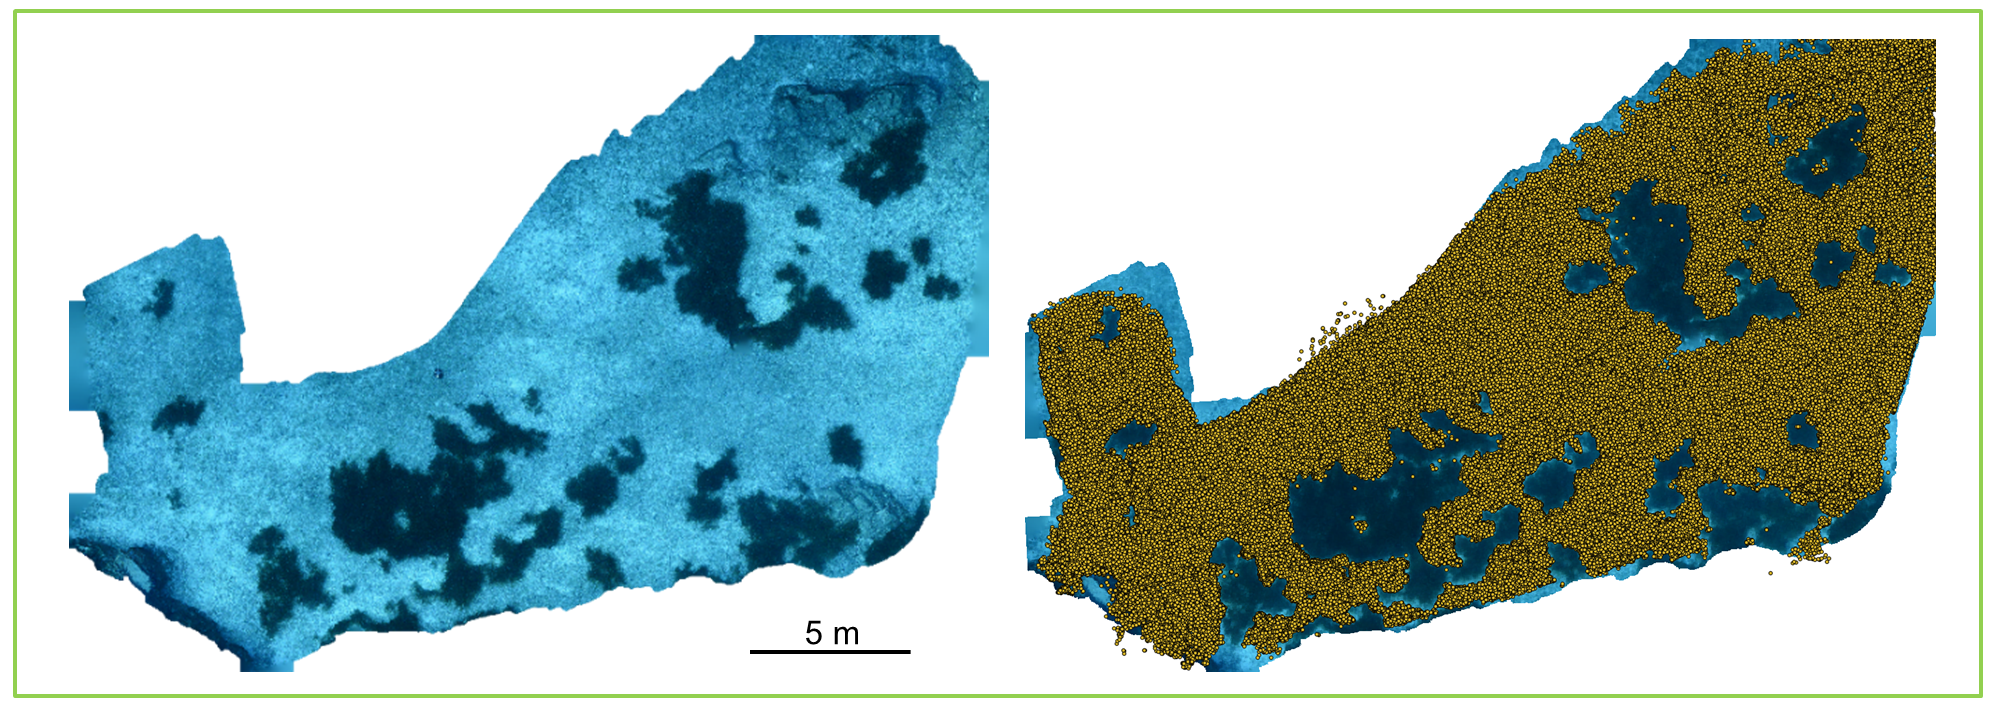
\includegraphics[width=\linewidth]{./5_chapitre3/Figure3.2}
		\caption[Visible \textit{Posidonia oceanica} patches in the sparse cloud after removing points with high reconstruction uncertainty.]{Visible \textit{Posidonia oceanica} patches in the sparse cloud after removing points with high reconstruction uncertainty (Cappo Rosso, Corsica, 2017).}
	\label{figure3.2}
\end{center}
\end{figure}

We performed 256 different classifications per site (with the previously cited values) in order to define the best set of parameters for the reconstruction uncertainty, resolution, closing size, and opening size. This corresponds to a total of 5376 classifications (256 combinations x 21 sites).

Our classification method used the sparse cloud as input (produced during bundle adjustment; see \autoref{figure3.3}). Though, the whole photogrammetric workflow was undertaken (i.e. bundle adjustment, point cloud densification, mesh building and texturing). This workflow was applied for each site in order to produce the orthomosaics. Indeed, these orthomosaics were necessary to manually digitalize the seagrass patches (used as ground truth to measure classification performances).

%%%%%%%%%%%%%%%%%%%%%%%%%%%%%%%%%%%%%%%%%%%%%
%%% Figure 3.3: Study sites TEMPO network %%%
%%%%%%%%%%%%%%%%%%%%%%%%%%%%%%%%%%%%%%%%%%%%%
\begin{figure}[H]
	\begin{center}
	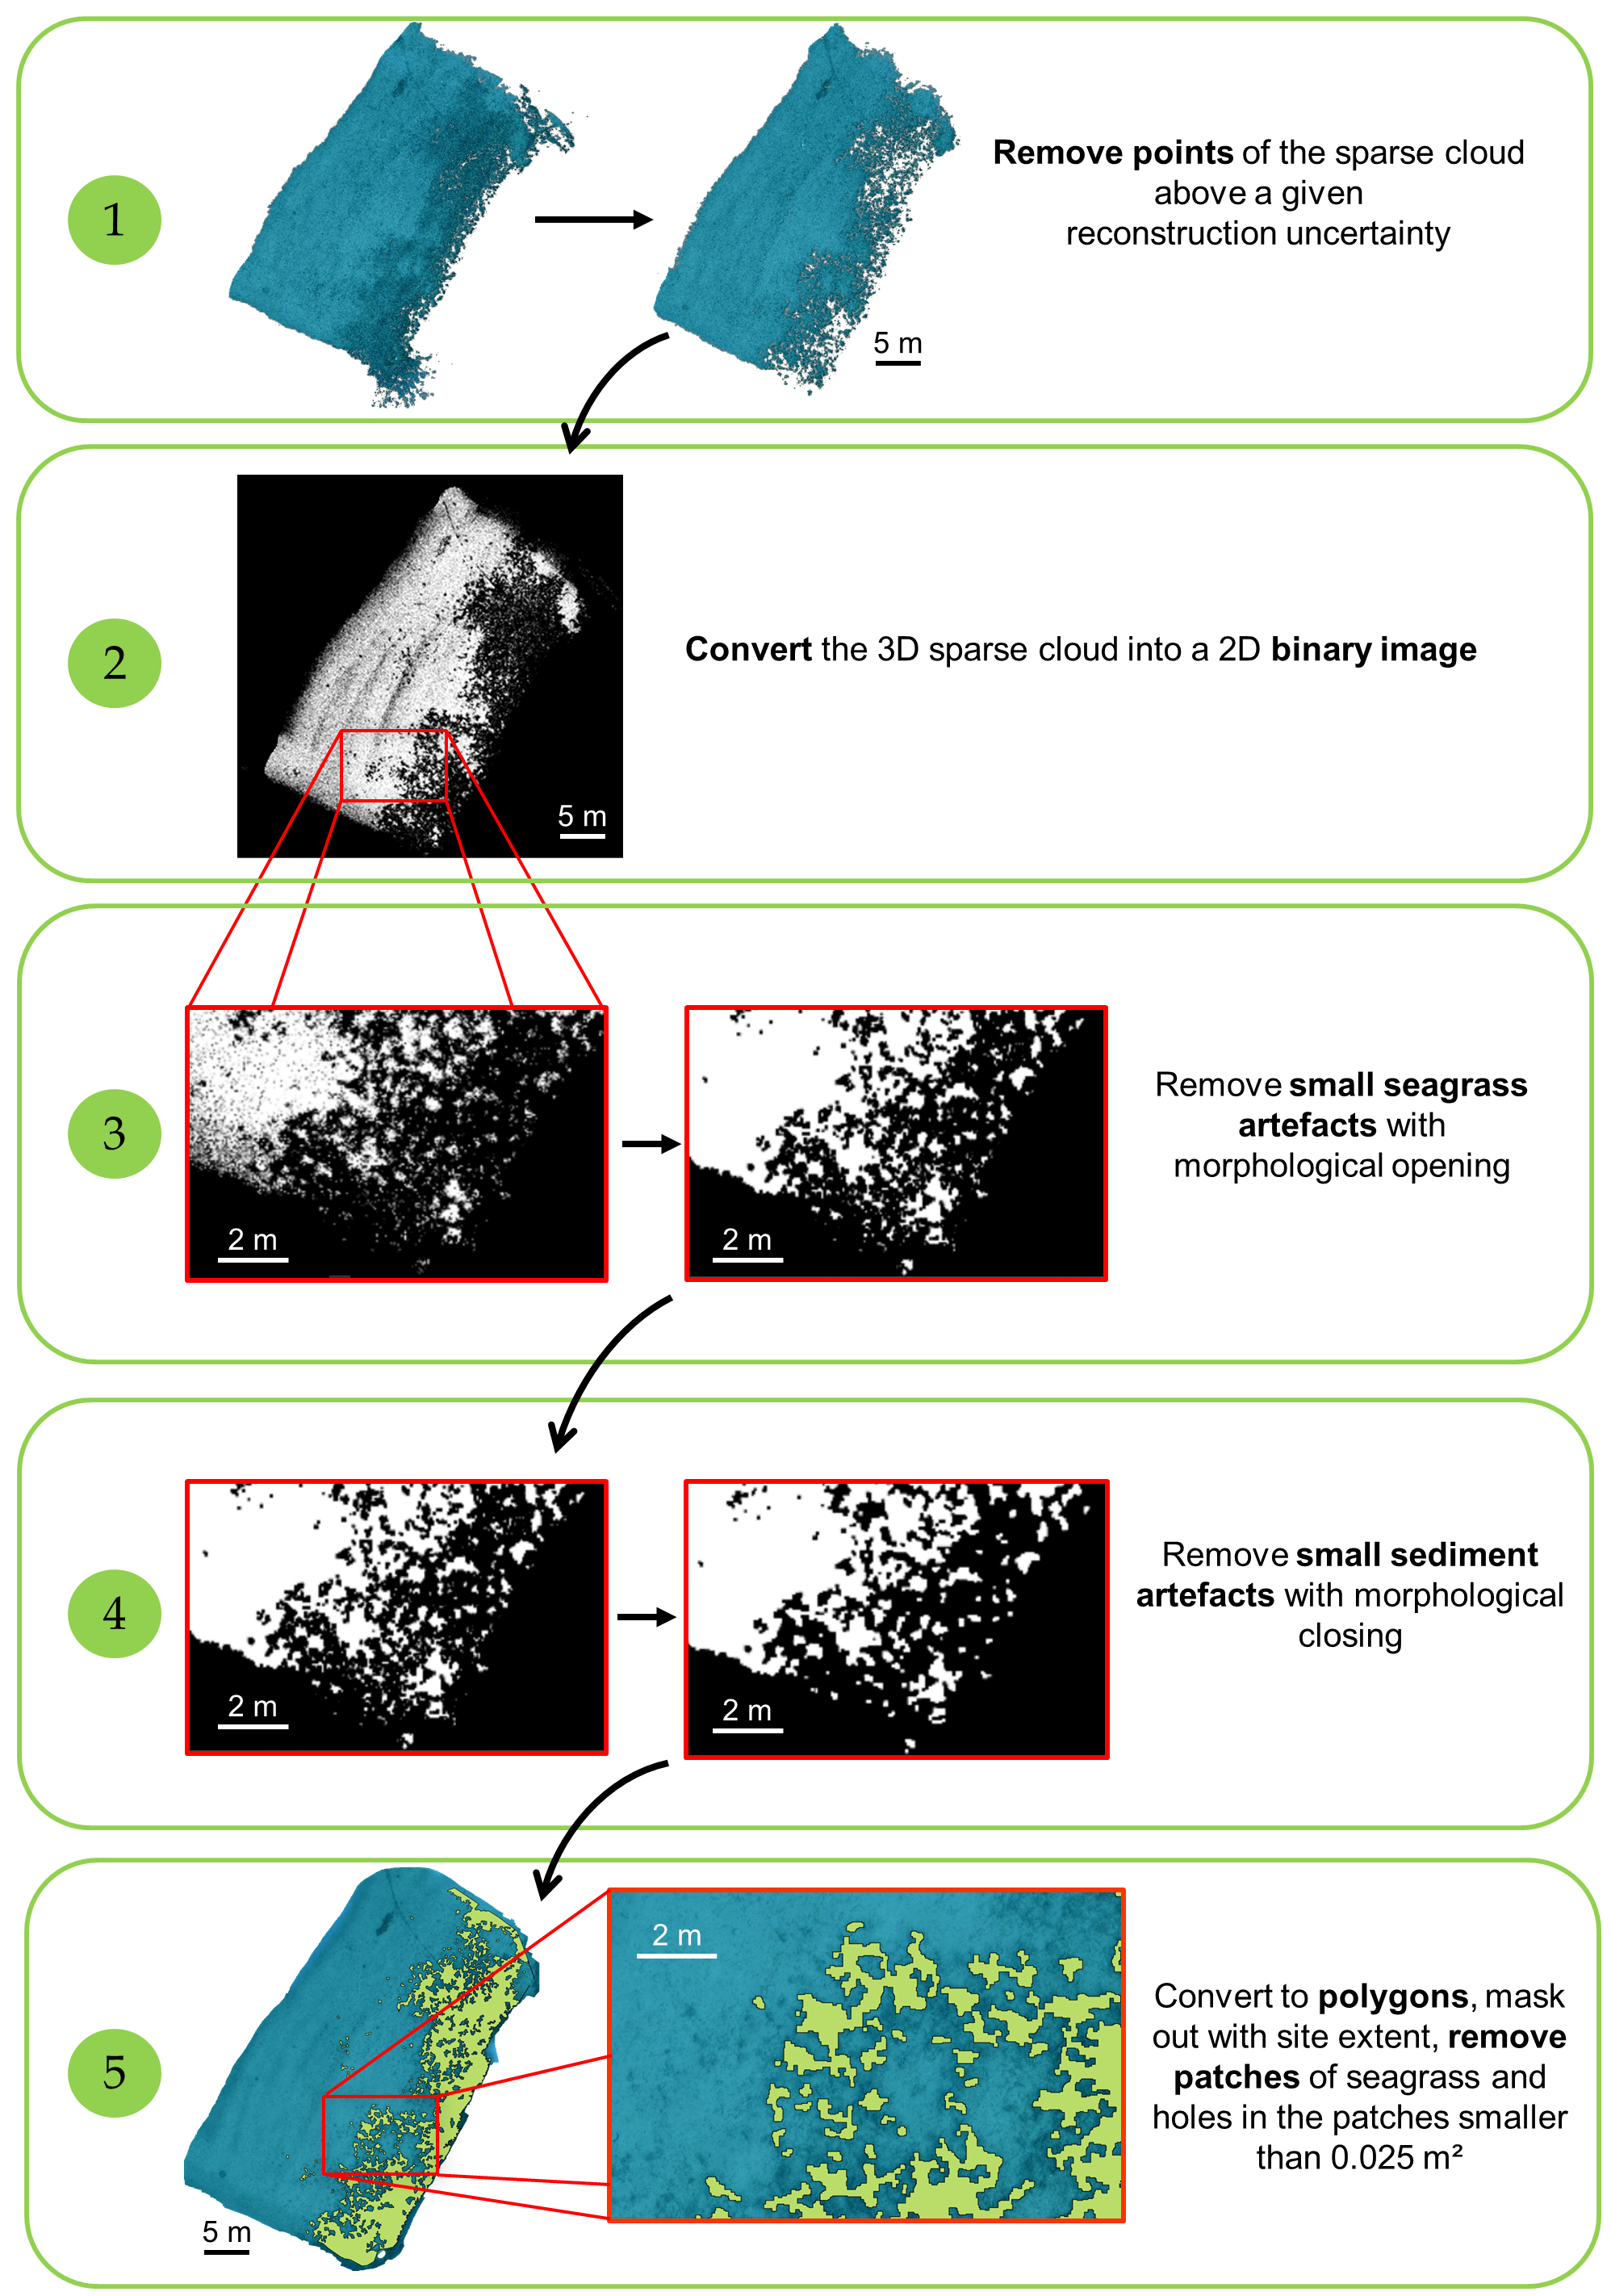
\includegraphics[width=\linewidth]{./5_chapitre3/Figure3.3}
		\caption[Workflow of the method.]{Workflow of the method.}
	\label{figure3.3}
\end{center}
\end{figure}

\subsection{Assessment of classification accuracy}
In order to assess the performance of the classification algorithm for each site, all \textit{P. oceanica} patches on the orthomosaic were digitized by hand. The accuracy of each classification was assessed by calculating the F1 score as follows:

\begin{equation}
\text{F1-score}=2\times\frac{\text{Precision}\times\text{Recall}}{\text{Precision}+\text{Recall}}
\end{equation}

\begin{equation}
\text{Precision}=\frac{\text{True Positive}}{\text{True Positive}+\text{False Positive}}
\end{equation}

\begin{equation}
\text{Recall}=\frac{\text{True Positive}}{\text{True Positive}+\text{False Negative}}
\end{equation}

With:

\begin{itemize}
\item \textbf{True positives:} pixels of \textit{P. oceanica} classified as \textit{P. oceanica};
\item \textbf{False positives:} pixels of sediment classified as \textit{P. oceanica};
\item \textbf{True negatives:} pixels of sediment classified as sediment;
\item \textbf{False negatives:} pixels of \textit{P. oceanica} classified as sediment.
\end{itemize}

The precision reflects the selectiveness of the method: a value of one means that all positives are true. The recall reflects the ability to detect \textit{P. oceanica}: a value of one means that all \textit{P. oceanica} pixels are detected and classified as such. F1 is an integrative indicator of both these measures, and ranges from zero to one, one being a perfect classifier.

In order to define the best parametrization over all study sites, we calculated the maximum F1 for each site and across all parametrizations. We then calculated the difference between each recorded F1 value and the calculated maximum F1 value for each site:

\begin{equation}
    F1diff_{i,s}=\max_i{F1_{i,s}}-F1_{i,s}
\end{equation}

With:
\begin{itemize}
\item $i$: combination of parameters
\item $s$: study site
\end{itemize}

In order to assess the true performance of the method, the accuracy for each site was calculated with the best parametrization defined over the remaining 20 sites. For a given site $s*$, the best combination of parameters was defined as minimizing the sum of these differences over all study sites except $s*$, i.e. the combination $i$, such as:


\begin{equation}
    \sum_{s-s*}{F1diff_{i,s}}=\min_i{\sum_{s-s*}{F1diff_{i,s}}}
\end{equation}

\subsection{Influence of the site properties on classification performances}
The method, which relies on the sparse cloud produced during bundle adjustment, could be affected by any factor altering image quality or tie point recognition:

\begin{itemize}
\item \textbf{Depth:} as depth greatly influences the amount of available natural light, it could affect the sparse cloud through a reduced image definition (higher ISO; greater aperture causing lower field of depth);
\item \textbf{Substrate type:} mud usually appears more homogenous than sand, it could affect tie point density and lead to false positives;
\item \textbf{Shoot density:} a low density could allow enough tie points to be recognized within the seagrass patches and lead to false negatives;
\item \textbf{Fragmentation:} a high fragmentation could affect classification performances by reducing the contrasts of tie point density in the sparse cloud, notably small holes in the seagrass could suffer from projected shadows of the neighbouring seagrass and produce false positives.
\end{itemize}

If the site surface area was not expected to influence the results of our methodology, its effect was tested anyway as it is expected to have a strong influence on the mapping resolution using acoustic telemetry.

The final F1s were analysed with regard to the properties of each site (depth, substrate, surface, fragmentation and shoot density). A Linear Model (LM) was built to assess the effect of each property on the F1 score. The LM initially incorporated all four properties, then was sequentially pruned by dropping the least significant property, such that the final LM included only those properties which had a significant effect on the F1 (t-test < 0.05). All analyses and calculations were performed with R Software V. 3.5.1 \citep{r_core_team_r:_2018}.

\subsection{Monitoring the evolution of \textit{P. oceanica} meadows}
Out of the 21 sites used for designing and parametrizing our methodology, three were monitored both in June 2016 and 2019 (“Cap Gros Nord”, “Cap Roux” and “Pointe Veille Est”), allowing for the assessment of temporal evolution of the lower limits. For these three sites, seagrass meadows were therefore mapped in 2016 and 2019, and measured progression and regression areas allowed calculating an evolution index as follows:

\begin{equation}
\text{Evolution Index}=\frac{\text{Progression - Regression}}{\text{Initial seagrass area}}
\end{equation}

This Evolution Index (EI) gives the proportion of net changes related to the initial seagrass area. Negative values correspond to a declining meadow while positive values reveal a progressing meadow.


% Results
\section{Results}\label{chapitre3_3}
Water conditions (salinity, temperature, turbidity) were homogenous during all acquisitions, and refraction was assumed constant over time and space as it has been proven to be insensitive to temperature, pressure and salinity \citep{moore_underwater_1976}. The total acquisition time for each site ranged between 12 to 68 minutes for a total number of photos of 480 to 2621. 

\subsection{Method accuracy}
F1 score ranged from 0.73 to 0.93 across the 21 sites, with a mean value of 0.84 (see \autoref{table3.2}). The lowest values corresponded to the sites with a very sparse limit (Carqueiranne, Rondinara, Pointe de la Calle), and the highest values corresponded to the sites with a sharp limit and dense meadow (Agay Ouest, Agriates, Cap Gros Nord). Precision ranged from 0.65 to 0.90, with a mean value of 0.79. Recall ranged from 0.70 to 1.00, with a mean value of 0.91.

%%%%%%%%%%%%%%%%%%%%%%%%%%%%%%%%%%%%%%%%%%%%%%%%%%%%%%%%%%%
%%% Table 3.2: Performance scores best parametrization  %%%
%%%%%%%%%%%%%%%%%%%%%%%%%%%%%%%%%%%%%%%%%%%%%%%%%%%%%%%%%%%
\begin{table}[H]
  \centering
  \normalsize
 % \raggedright
  \caption[Performance scores corresponding to the best parametrization for each site.]{Performance scores corresponding to the best parametrization for each site. Unc. = Reconstruction Uncertainty}
  \label{table3.2}
    \begin{tabular}{*{1}{c}|*{4}{c}|*{3}{c}}
        \toprule
        \textbf{} & \multicolumn{4}{c}{\textbf{Best parametrization}} & \multicolumn{3}{c}{\textbf{Performance scores}} \\ 
        \midrule
        \textbf{Site} & \textbf{Unc.} & \makecell{\textbf{Resolution} \\ \textbf{(m)}} & \makecell{\textbf{Closing} \\ \textbf{Size (pix)}} & \makecell{\textbf{Opening} \\ \textbf{Size (pix)}} & \textbf{Precision} & \textbf{Recall} & \makecell{\textbf{F1} \\ \textbf{score}} \\
        \midrule
        Agay Ouest & 10 & 0.02 & 5 & 4 & 0.85 & 0.96 & 0.90 \\
        Agriates & 10 & 0.02 & 5 & 4 & 0.90 & 0.95 & 0.93 \\
        Cap Gros Nord & 10 & 0.02 & 5 & 4 & 0.90 & 0.96 & 0.93 \\
        Cap Roux & 10 & 0.02 & 5 & 4 & 0.81 & 0.94 & 0.87 \\
        Cappo Rosso & 10 & 0.02 & 5 & 4 & 0.72 & 1.00 & 0.84 \\
        Carqueiranne & 10 & 0.02 & 5 & 4 & 0.67 & 0.81 & 0.73 \\
        Giraglia & 10 & 0.03 & 3 & 3 & 0.84 & 0.92 & 0.87 \\
        Golfe Santa Manza & 12 & 0.03 & 3 & 4 & 0.86 & 0.70 & 0.77 \\
        Isolella & 10 & 0.02 & 5 & 4 & 0.79 & 0.97 & 0.87 \\
        Murtoli & 10 & 0.02 & 5 & 4 & 0.70 & 1.00 & 0.82 \\
        Paulilles & 10 & 0.02 & 5 & 4 & 0.65 & 0.90 & 0.76 \\
        Plage Suveret & 10 & 0.02 & 5 & 4 & 0.78 & 0.98 & 0.87 \\
        Plage Trottel & 10 & 0.02 & 5 & 4 & 0.69 & 0.99 & 0.82 \\
        Pointe de la Calle & 10 & 0.03 & 3 & 3 & 0.73 & 0.75 & 0.74 \\
        Pointe Rube & 10 & 0.02 & 5 & 4 & 0.78 & 0.98 & 0.87 \\
        Pointe Veille Est & 10 & 0.02 & 5 & 4 & 0.83 & 0.99 & 0.90 \\
        Presqu’île de Giens & 10 & 0.02 & 5 & 3 & 0.78 & 0.84 & 0.81 \\
        Punta Mortella & 10 & 0.03 & 3 & 3 & 0.79 & 0.86 & 0.83 \\
        Punta Vaccaja & 10 & 0.02 & 5 & 4 & 0.75 & 0.95 & 0.84 \\
        Rondinara & 12 & 0.03 & 3 & 4 & 0.84 & 0.70 & 0.76 \\
        Sardinaux & 10 & 0.03 & 3 & 3 & 0.83 & 0.94 & 0.89 \\
        \midrule
         &  &  &  & \textbf{Mean} & \textbf{0.79} & \textbf{0.91} & \textbf{0.84} \\ \bottomrule
    \end{tabular}
\end{table}

The combination of parameters that gave the best results over all sites (minimizing equation 5 across all sites) was: uncertainty threshold = 10, resolution = 0.02 m, closing size = 5 pix and opening size = 4 pix. For this parametrization, over the 21 sites, the mean precision, recall, and F1 were: 0.78, 0.92 and 0.84, respectively. \autoref{figure3.4} illustrates classification results with different fragmentation levels.

%%%%%%%%%%%%%%%%%%%%%%%%%%%%%%%%%%%%%%%%%%%%%%
%%% Figure 3.4: Results with fragmentation %%%
%%%%%%%%%%%%%%%%%%%%%%%%%%%%%%%%%%%%%%%%%%%%%%
\begin{figure}[htbp]
	\begin{center}
	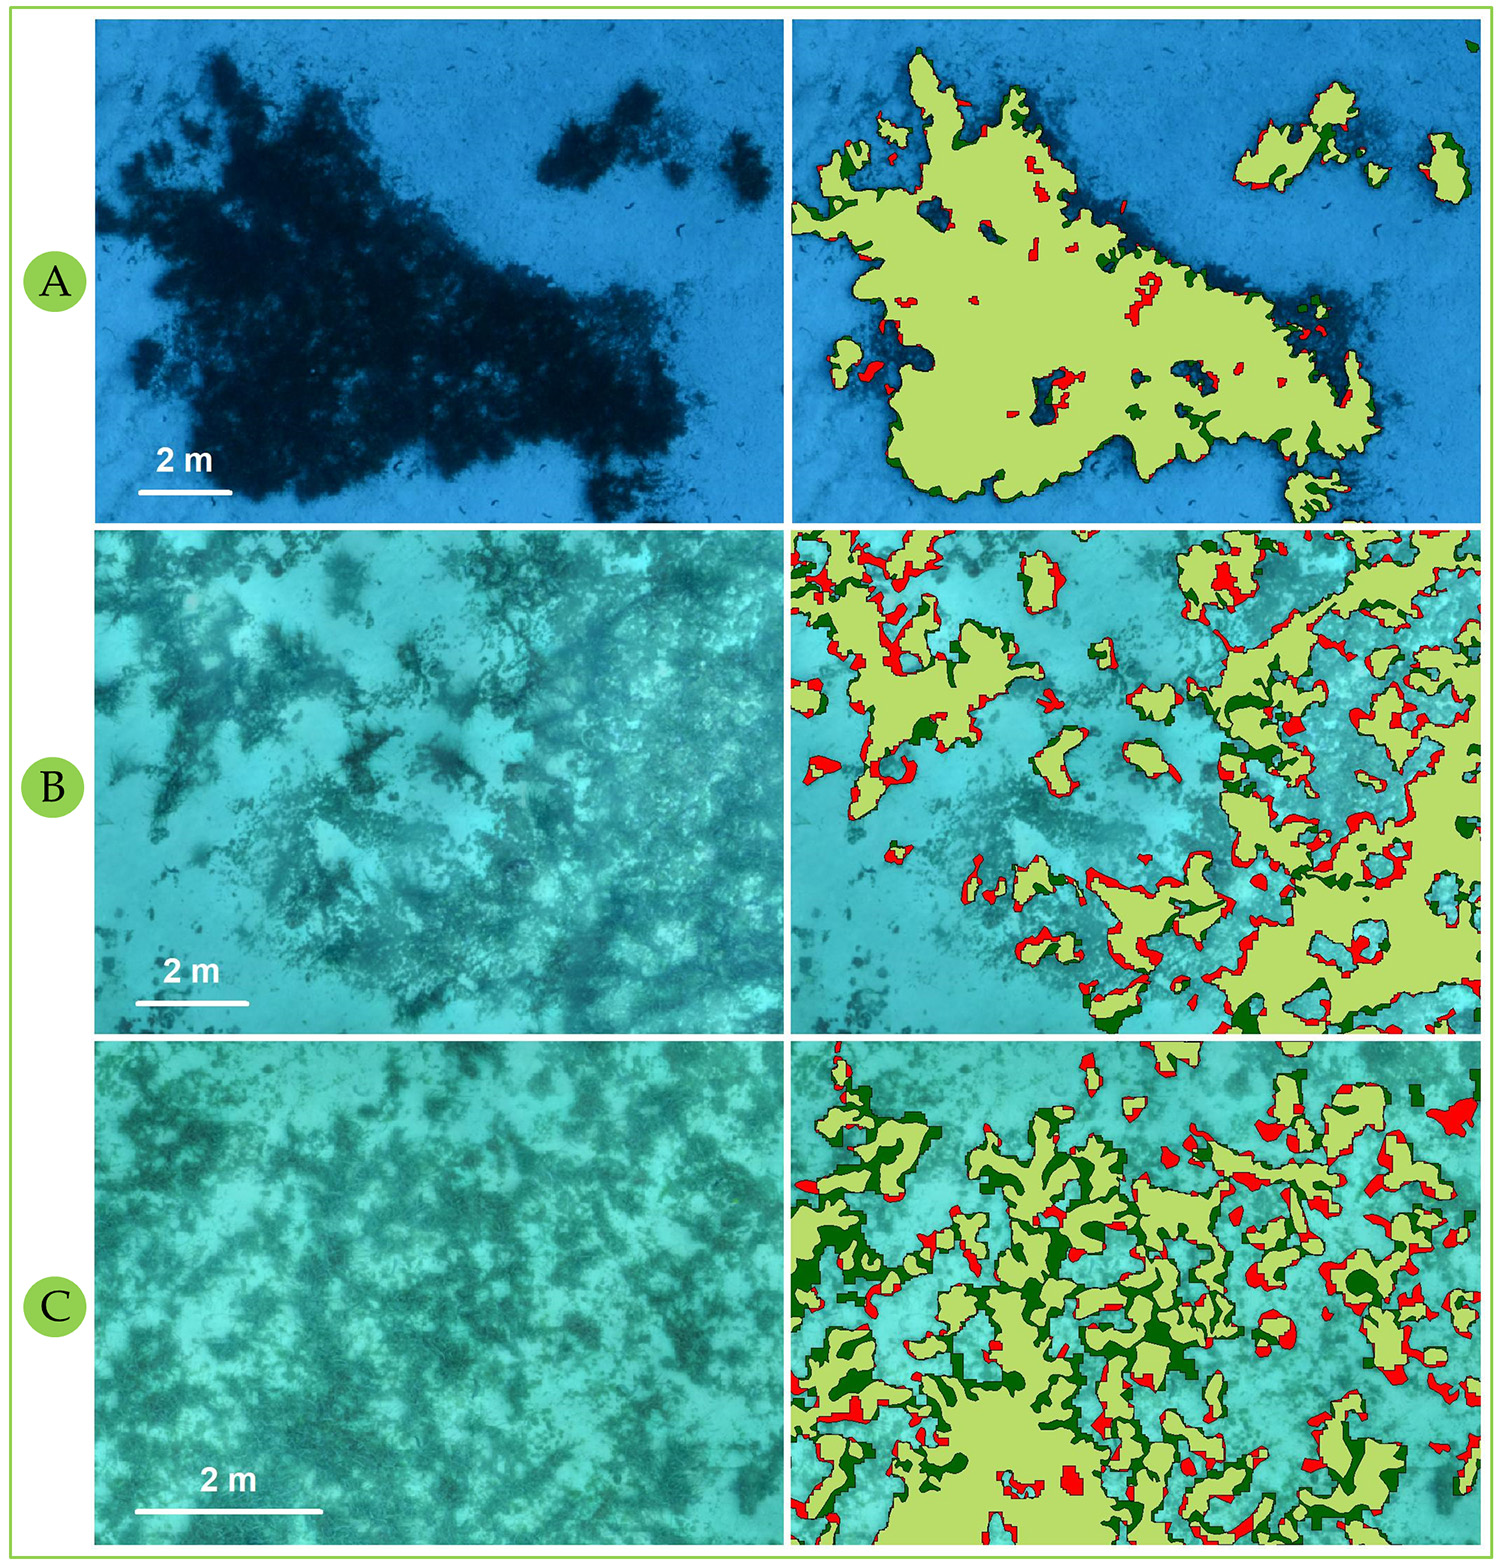
\includegraphics[width=\linewidth]{./5_chapitre3/Figure3.4}
		\caption[Classification results for three levels of fragmentation.]{Classification results for three levels of fragmentation. Orthomosaic (left) and results of the classification (right). (A) Agriates, fragmentation = 2.43, F1 = 0.93; (B) Presqu’île de Giens, fragmentation = 5.10, F1 = 0.81; (C) Carqueiranne, fragmentation = 12.30, F1 = 0.73. Light green = true positives; dark green = false positives; red = false negatives; no colour = true negatives.}
	\label{figure3.4}
\end{center}
\end{figure}

\subsection{Influence of the site properties on classification performances}
The depth, substrate, surface, and shoot density had no effect on the F1 score (t-test, p > 0.05). Only fragmentation had a significant negative effect on the F1 score (F1 = -0.017 * fragmentation, R² = 0.50; t-test, p < 0.001). The method proved highly accurate (F1 > 0.8) in various, adverse conditions, including the presence of dead matte (i.e. what remains after the death of \textit{Posidonia oceanica}; see \autoref{figure3.4} B - C) or dead \textit{Posidonia oceanica} litter (Agriates, Giraglia; see \autoref{figure3.5}). 

%%%%%%%%%%%%%%%%%%%%%%%%%%%%%%%%%%%%%%%%%%%%%
%%% Figure 3.5: Study sites TEMPO network %%%
%%%%%%%%%%%%%%%%%%%%%%%%%%%%%%%%%%%%%%%%%%%%%
\begin{figure}[H]
	\begin{center}
	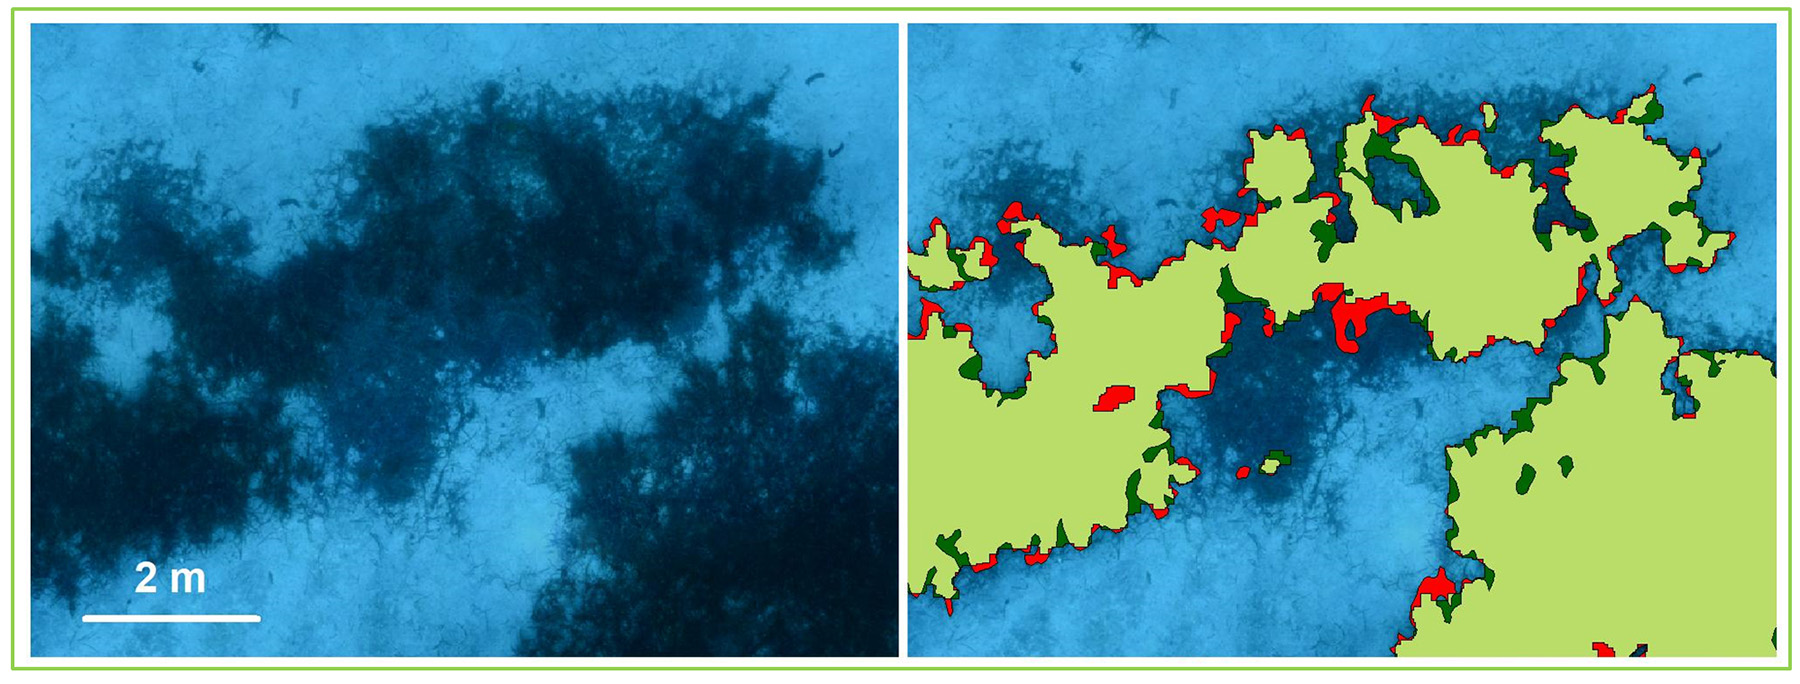
\includegraphics[width=\linewidth]{./5_chapitre3/Figure3.5}
		\caption[Zoom on dead \textit{P. oceanica} litter patches.]{Zoom on dead \textit{P. oceanica} litter patches (Giraglia, F1 = 0.87). Light green = true positives; dark green = false positives; red = false negatives; no colour = true negatives.}
	\label{figure3.5}
\end{center}
\end{figure}


\subsection{Monitoring the evolution of \textit{P. oceanica} meadows}
Evolution Index was positive for the three sites, with values ranging from 8 \% to 46 \%; progression ranged from 7.71 to 11.07 m², and regression from 0.25 to 2.60 m² (see \autoref{table3.3}). \autoref{figure3.6} shows the orthomosaics of the three sites along with the localization of the stable seagrass, progression and regression.

%%%%%%%%%%%%%%%%%%%%%%%%%%%%%%%%%%%%%%%%%%%%%%%%%%%%%%%%%%%%%%%%%%%%%
%%% Table 3.3: Evolution of 3 lower limits between 2016 and 2019  %%%
%%%%%%%%%%%%%%%%%%%%%%%%%%%%%%%%%%%%%%%%%%%%%%%%%%%%%%%%%%%%%%%%%%%%%
\begin{table}[htbp]
  \centering
  \normalsize
 % \raggedright
  \caption[Evolution of three \textit{P. oceanica}’s lower limit between 2016 and 2019.]{Evolution of three \textit{P. oceanica}’s lower limit between 2016 and 2019.}
  \label{table3.3}
    \begin{tabular}{*{6}{c}}
        \toprule
        \textbf{Site} & \makecell{\textbf{Stable} \\ \textbf{seagrass (m²)}} & \makecell{\textbf{Stable} \\ \textbf{substrate (m²)}} & \makecell{\textbf{Progression} \\ \textbf{(m²)}} & \makecell{\textbf{Regression} \\ \textbf{(m²)}} & \makecell{\textbf{Evolution} \\ \textbf{Index (\%)}} \\ \midrule
        Cap   Gros Nord & 51.73 & 51.99 & 10.70 & 2.60 & 15 \\
        Cap   Roux & 23.23 & 27.17 & 11.07 & 0.25 & 46 \\
        Pointe   Veille Est & 61.51 & 38.73 & 7.71 & 2.50 & 8 \\ \bottomrule
    \end{tabular}
\end{table}

%%%%%%%%%%%%%%%%%%%%%%%%%%%%%%%%%%%%%%%%%%%%%
%%% Figure 3.6: Study sites TEMPO network %%%
%%%%%%%%%%%%%%%%%%%%%%%%%%%%%%%%%%%%%%%%%%%%%
\begin{figure}[H]
	\begin{center}
	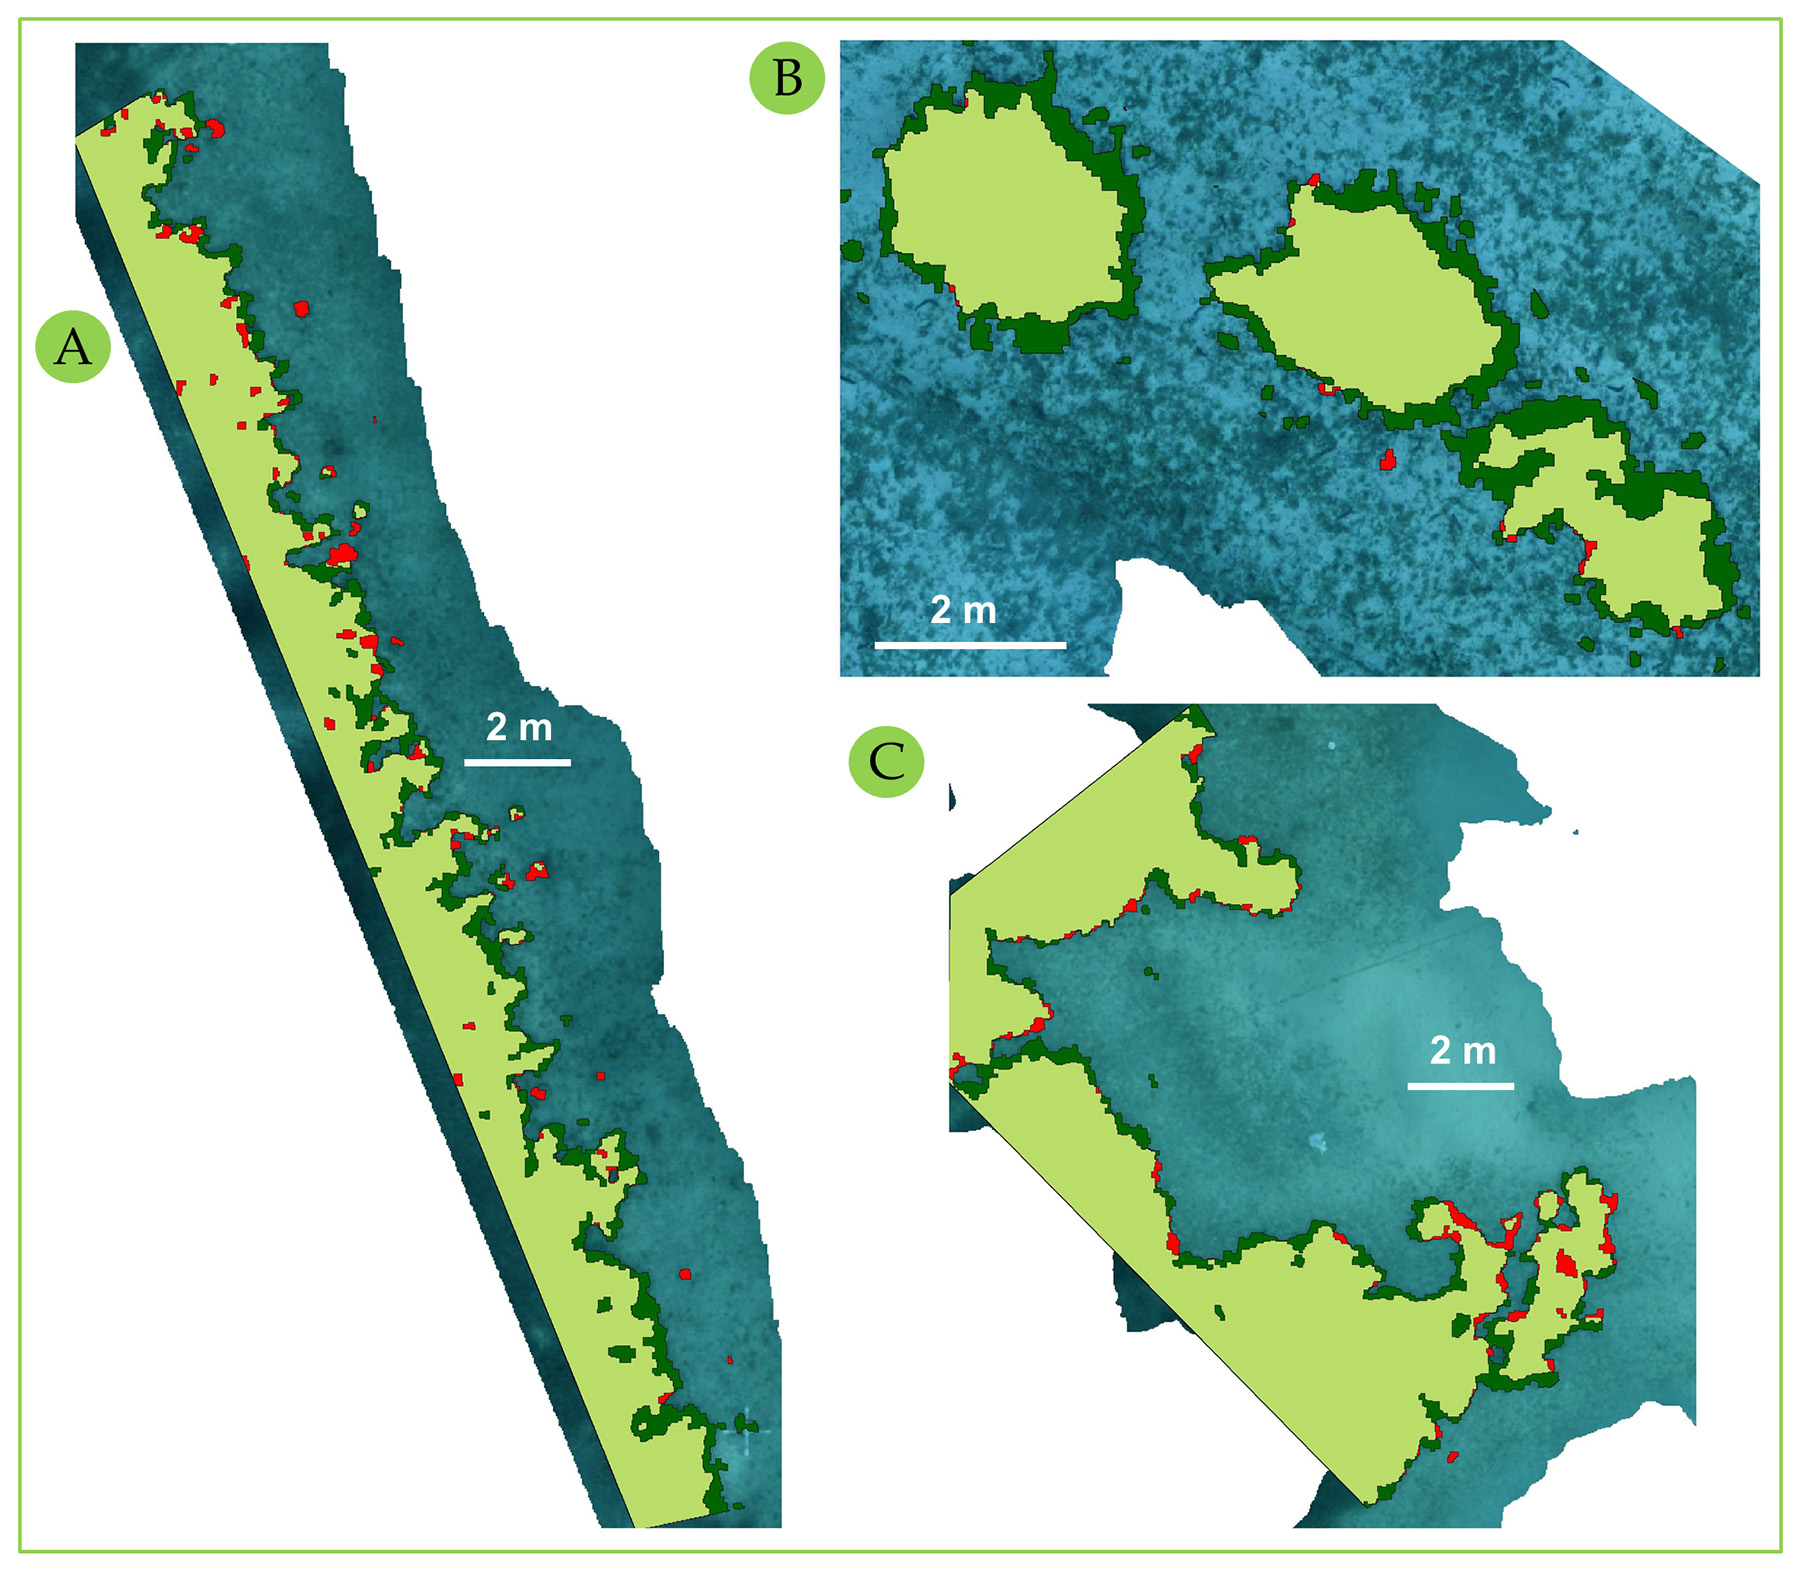
\includegraphics[width=\linewidth]{./5_chapitre3/Figure3.6}
		\caption[Evolution of the Posidonia oceanica’s lower limit on three study sites between 2016 and 2019.]{Evolution of the Posidonia oceanica’s lower limit on three study sites between 2016 and 2019. A = “Cap Gros Nord” ; B = “Cap Roux” ; C = “Pointe Veille Est”. Light green = stable meadow ; Dark green = progression ; Red = regression.}
	\label{figure3.6}
\end{center}
\end{figure}

\newpage

% Discussion
\section{Discussion}\label{chapitre3_4}
This study aimed to develop a simple and operational methodology, which is automatic, efficient, and reproducible, for fine-scale mapping of up to 1000 m² \textit{Posidonia oceanica} seagrass beds, with various morphologies and in different lighting conditions.

\subsection{Performances and limits of the methodology}
It should be noted that previous single-site studies have performed better than our own study (95 \% for \textit{P. oceanica} patches on a rocky substrate and similar resolution \citep{bonin-font_towards_2016}). Yet, with an F1 score = 0.73 – 0.93, the method proved to be moderately to highly accurate, performing successfully in 21 morphologically different sites, which varied in terms of their substrate, surface, depth, shoot density, and fragmentation, and in various acquisition conditions where light and water clarity were not always optimal. The method, which relies on the sparse cloud produced during bundle adjustment, could be affected by any factor altering image quality or tie point recognition. However, the results showed that, within the range of tested conditions, the only factor that had a significant effect on the F1 measure was fragmentation (t-test, p-value < 0.001). Nonetheless, highly fragmented lower limits are also difficult to map with acoustic telemetry, which relies on the diver ability to map all small patches and details of the limit within a limited amount of time. For the same reason, surface area is also expected to have a strong influence on the mapping resolution using acoustic telemetry, while it had no effect on the classification performances of our method (t-test, p-value > 0.05).

The high recall values (0.70 – 1.00, mean 0.91) indicate that our classifier detected a very large proportion of the existing seagrass (large quantity of true positives compared to that of false negatives). Yet, the lower values of precision (0.65 – 0.90, mean 0.79) suggest that part of the substrate was recognized as seagrass (false positives). Although the performance of the classifier is satisfying (high F1 scores), still the method could slightly overestimate the presence of \textit{P. oceanica} in some cases. By means of comparison, although this study was conducted at a much larger scale (~100 km² vs 1000 m²) and resolution (30 m vs 0.02 m), the remote sensing method developed by Topouzelis et al. (2018) reached a mean F1 of 0.36 (mean accuracy of 0.76) on 62 different Natura 2000 sites in Greece. Our method, which uses seagrass movement and texture homogeneity to its own advantage, proved highly accurate even in the presence of dead matte or dead litter which could easily have mislead a classification algorithm based on colour or luminance. This particular aspect matters as health assessment and ecological indices based on seagrass surfaces require distinguishing dead from living \textit{P. oceanica}. The method was largely unaffected by the substrate type with good results collected on both sand and mud, but was adversely affected by the fragmentation of the meadow. However, the ground truth of this study relied on manually drawn \textit{P. oceanica} maps based on orthomosaics of the sites. Further studies should address this issue and assess the bias in the ground truth by repeating the drawings made of each site by several experts. 

One possible drawback of this methodology is its limited ability to discriminate between classes of seagrass or macroalgae. The risk is that anything which slightly resembles \textit{P. oceanica} in appearance (homogenous texture; moves in the current) will also have a low point cloud density and high reconstruction uncertainty, and could consequently be misrecognized by the algorithm as \textit{P. oceanica}. However, this case has not been observed across our study sites. Further investigations could tackle this issue by utilizing both reconstruction uncertainty and another property, such as colorimetry or roughness. Conversely, the limited discriminatory capacity of this method could render it suitable for monitoring other species of seagrass or seaweed (Zostera, Cymodocea, kelp, etc) without having to make any major, methodological adjustments.

\subsection{Application of the methodology within a monitoring network}
There is currently no alternative to acoustic telemetry for fine-scale studies of seagrass meadows’ lower limit. However, the mapping technique developed in this study proved to be accurate, repeatable, and operational in various conditions, and is therefore a viable alternative. Data acquisition requires no particular skillset: a single camera (monoscopic photogrammetry) and a competent diver. Processing the raw data to produce the map is a fully automated procedure, reducing the time required by a human analyst. In terms of processing time, the photogrammetric method proposed had the comparative advantage of being time-effective. It makes use of only the first (and shortest) step of the photogrammetric workflow (< 60 min processing); namely, bundle adjustment. Acquisition time is relatively short (12 - 68 min) and insensitive to the fragmentation level when using underwater photogrammetry; conversely, the time required to manually pinpoint the lower limits of the seagrass with acoustic telemetry (one point every 40 cm in average \citep{descamp_fast_2011}) is greatly affected by the size and fragmentation level of the meadow. An acoustic telemetry device is generally far more expensive than a single digital camera, and the level of detail achieved is entirely dependent upon diver willingness. Furthermore, even in the most complex configurations and notably highly fragmented limits where our results showed a lower accuracy, it is still possible to use the orthomosaics produced with underwater photogrammetry to manually digitalize the meadows.

With acquisitions on three sites in both 2016 and 2019, we could apply our method for the assessment of the ecological status of these limits with an Evolution Index based on the net progression of the meadow. We showed that “Cap Gros Nord”, “Cap Roux” and “Pointe Veille Est” were progressive over the period 2016 – 2019 (EI = 15 \%, 46 \% and 8 \%, respectively). The application of the method on these three sites proved its operability, but linking these evolutions with anthropogenic pressures and provide decision makers with good understanding of the evolution at the regional scale  requires a large number of monitored sites \citep{marba_mediterranean_2014, holon_impact_2015, de_los_santos_recent_2019}. Thanks to the low amount of time required underwater and the satisfying classification performances, our method seems suited for its use in a dense large scale monitoring system.

Consequently, this method provides a true alternative to acoustic telemetry for fine-scale mapping of living \textit{P. oceanica}, and could be applied in the study of other submerged aquatic vegetation (seagrass, seaweed species), and habitats such as coral or coralligenous reefs, which are threatened by the colonization of certain algae species. In sum, our method enables the production of numerous seagrass maps over a short period of time, and time effectiveness is vitally important to ensure the successful operation of a large monitoring network such as TEMPO network \citep{andromede-oceanologie_tempo_2020}.
